
%*******************************************************
% Chapter 1
%*******************************************************

\myChapter{Kolmogorov axioms}

\begin{refsection}

   Rigorous foundation of mathematical probability is provided by
   Kolmogorov's measure-theoretical approach%
   \footcite{Kolmogorov:1956}.
   In this framework, the mathematical notion of probability is defined in an abstract way by 
   all and only the rules that any probability must fulfill.
   Among the strenghts of this approach is the fact that it 
   completely \emph{decouples} the definition of probability from empirical
   notions and conceptual interpretations. 
   Kolmogorov's axioms provides the rules of the game, allowing to establish
   properties of probability and ways to manipulate mathematical
   probabilities on a general ground, without relying on a specific way to
   assign values to a probability. 
   In order to apply the theory to study a particular situation, one should supply the
   framework with a concrete ``probabilistic model''
   (\ie, she/he should assign a probability)
   suitable for the example at hand; the choice and the construction of the
   probabilistic model is an empirical ``input'' which should be provided
   externally to
   the Kolmogorov framework.

   It is worth mentioning that Kolmogorov's approach to mathematical
   probability is not free from criticism. 
   An introductory review of approaches to probability and their conceptual
   interpretation 
   are  briefly sketched
   in \cref{sec:other_probability}.

   \begin{figure}
\centering
\subfloat[][]{%
   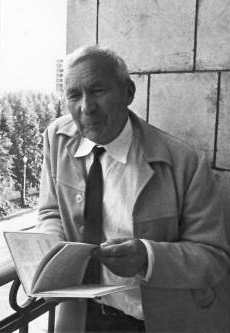
\includegraphics[width=.45\columnwidth]{Kolmogorov}%
   \label{fig:kolmogorov}%
}
\quad
\subfloat[][]{%
   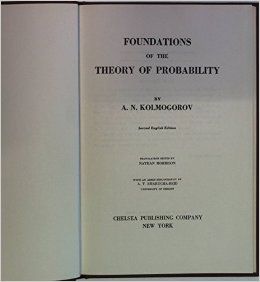
\includegraphics[width=.45\columnwidth]{Kolmogorov_book}%
   \label{fig:kolmogorov_book}%
}
\caption{%
   \protect\subref{fig:kolmogorov} Russian mathematician Andrey Nikolaevich Kolmogorov
   (1903--1987). Source: Wikipedia.
   \protect\subref{fig:kolmogorov_book} Title page of english edition of
   Kolmogorov's \emph{Foundations of the theory of probability}.
}
\end{figure}

\section{Crash course in abstract measure theory}

Kolmogorov axioms are rooted in abstract measure theory.
Since this is a fairly advanced topic in mathematics, we give here a brief
account of the very basic of this subject in order the Reader to be accustomed
to it at least to some extend%
\footcite[For a more comprehensive treatment and its application to rigorous
probability, refer to, \eg,
][]{Kolmogorov:1956,Billingsley:1995,Rosenthal:2006}.

Roughly speaking, the ultimate goal is that of  appending some reasonable
notion of ``measure'' to the subsets of a given non-empty set (the precise mathematical definition of
measure coming 
soon). Troubles eventually arises however when dealing with sets having
uncountable many items if one tries to apply the notion of measure naively to
all subsets of such sets. The famous Banach-Tarsky paradox
is the  prototype of the  kind of difficulties one encounters.

\begin{approfondimento}
For those who are not familiar, a discussion of the Banach-Tarsky
paradox can be found, \eg, in \cite{Stromberg:1979}
and references therein. 
Proof of Banach-Tarsky paradox is highly non-trivial and it relieas technically on  the axiom of
choice. 
Nevertheless, the statement of the theorem itself is paradigmatic on the kind
of difficulties one meets when dealing with uncountable sets.
\end{approfondimento}


   To overcome the aforementioned difficulties when trying to ``measure'' a subset of a set, at a techical level one resorts to constrain
the definition of 
``measure'' over suitable collections of subsets called $\sigma$-algebras. 

Let 
$\Omega$ be any set.
Hereafter, $2^{\Omega}$ will denote the ``power set'' of $\Omega$, \ie, 
the set of 
   all and only the subsets of
   $\Omega$. 
   In
   axiomatic set theory, the existence of $2^{\Omega}$ for every set $\Omega$
   is a postulate%
   \footnote{The axiom of power set is one of the Zermelo-Fraenkel axioms. It allows a simple definition of the Cartesian product of two sets, which in turn allows to define the notion of application between sets.}.


\begin{definition}[$\sigma$-algebra]
	Let $\Omega$ be any \emph{non-empty} set and 
   $\Sigma \subseteq 2^{\Omega}$ any arbitrary subset of the power set.
	$\Sigma$ is called 
	a $\sigma$-algebra over
   $\Omega$ if 
   \begin{enumerate} [label=(\alph*)]
      \item\label{item:sigma1} $\Omega \in \Sigma$;
      \item\label{item:sigma2} for every $A \subseteq \Omega$, if $A \in \Sigma$ then $
	 \complement{A}{\Omega}\in \Sigma$;
      \item\label{item:sigma3}for every sequence
	 $\fullfunction{(A_{n})_{n\in\N}}{\N}{\Sigma}$ of subsets of $\Omega$
	 belonging to $\Sigma$,
	 $\bigcup_{n\in\N} A_{n} \in \Sigma$.
   \end{enumerate}
\end{definition}

In words:
\ref{item:sigma1} implies that any $\sigma$-algebra is \emph{non-empty}.
\ref{item:sigma2} means a $\sigma$-algebra is closed under the
complementation: if an arbitrary subset $A$ belongs to $\Sigma$ then also its complementary $\complement{A}{\Omega}$ belogs to it. 
\ref{item:sigma3}  means that the $\sigma$-algebra is closed under
\emph{countable}
unions. 
This latter assumption might look rather technical at this level.
Why not just restrict ourselves to the union of a \emph{finite} (instead of countably infinite) number of subsets?
As we shall see later, \ref{item:sigma3} 
allows 
to handle convergence theorems, to take limits of sequences of subsets,  etc. 

   \begin{remark}
   The empty set $\varnothing$ also belongs to any $\Sigma$-algebra. 
	   Proof: 
by 
\ref{item:sigma1} $\Omega$ belongs to $\Sigma$;
	   \ref{item:sigma2}, its complement $\complement{\Omega}{\Omega} = \varnothing$ must belong to 
$\Sigma$. 
\end{remark}

\begin{example}
	Given any set $\Omega$, 
   the subset $\Set{\Omega, \varnothing}\subseteq2^{\Omega}$ consisting only of the empty set
   $\varnothing$ and the set $\Omega$ itself is a $\sigma$-algebra over $\Omega$; it is called
   the ``minimal''
or ``trivial'' $\sigma$-algebra over $\Omega$.
\end{example}
\begin{example}
   Let $\Omega$ be a non-empty set having a non-trivial subset
   $A\subseteq\Omega$.
   The subset $\Set{\Omega, A, \complement{A}{\Omega},
      \varnothing}\subseteq2^{\Omega}$ 
   is a $\sigma$-algebra over $\Omega$.
\end{example}

\begin{example}
   The power set $2^{\Omega}$ of a set $\Omega$ is a $\sigma$-algebra over
   $\Omega$, called
   the ``discrete'' $\sigma$-algebra.
\end{example}

A set endowed with a sigma algebra is called a ``measurable space''; the reason
for this name is that it is always possible to define a ``measure'' on it.
More formally, we have the following definition.

\begin{definition}[Measurable space]
   An ordered pair $(\Omega, \Sigma)$ where $\Omega$ is an arbitrary set and
   $\Sigma$ is any $\sigma$-algebra over $\Omega$ is  called 
   a ``measurable space''.
\end{definition}

\begin{lemma}
   Let $(\Omega, \Sigma)$ be any measurable space.
   Then, for every sequence $\fullfunction{(A_{n})_{n\in\N}}{\N}{\Sigma}$ of
   elements in the $\sigma$-algebra $\Sigma$, we have
   \begin{dmath*}
      \bigcap_{n\in\N} A_{n} \in \Sigma
   \end{dmath*},
   \ie, any $\sigma$-algebra is also closed with respect to countable
   intersection.
\end{lemma}
\begin{proof}
   DeMorgan rules + induction.
\end{proof}


   \section{Set theory definition of probability}
   

   Dice: \drawdie{1} 

   \section{First properties of probability}

   \begin{figure}
      \centering
      \begin{venndiagram2sets}[overlap=-1cm,labelNotAB={$\Omega$}]
	 \fillACapB
      \end{venndiagram2sets}
      \caption{Union}
   \end{figure}


   \section{Borel-Cantelli lemmas}

   \section{Discrete probability space}


   Before continuing with the discussion of probability measures in
   their full generality, it is helpful to consider the simpler case where the
   sample
   space $\Omega$ is finite or countable.

   \subsection{Dices}

   \subsection{Urns}

   \subsection{Coupon collector problem}
   
   \section{Bertrand paradox}

   \section{Conditional probabilities and independent events}


   \begin{definition}[Conditional probability]
      \label{def:conditional_probability}
      Let $(\Omega, \Sigma, \P{\cdot})$ be a probability space and $A,B\in
      \Sigma$ such that $\P{B} > 0$. The ``conditional probability of $A$ given
      $B$ is defined as 
      \begin{dmath}
	 \P{A\given B}  \coloneqq \frac{\P{A \cap B }}{\P{B}}
      \end{dmath}.
   \end{definition}

   \begin{remark} 
      The definition makes sense since $A,B \in \Sigma$ implies $A\cap B\in
      \Sigma$ (being $\Sigma$ a $\sigma$-algebra).
      The condition $\P{B} > 0$ is required otherwise the denominator on the
      right-hand side would vanish.
   \end{remark}

 Set interpretation of 
      \cref{def:conditional_probability}:
      $\P{A\given B}$ can be visualized as if we were restricting the sample
      space to the subset $B$ alone. The logic
      behind this equation is that if the outcomes are restricted to B, this
      set serves as the new sample space.

   \section{Bayes' theorem}


%   \begin{advanced}
%      \section{Bayes theorem made simple using LEGO bricks}
%   \end{advanced}
%
%   This section is inspired by a online blog from Will Curt%
%   \footcite{Onl-curt:2015}.

   \section{A panorama of approaches to probability}
   \label{sec:other_probability}


   No attempt will be make at discussing the deep philosophical  implications
of applying the Kolmogorov's framework.

A review is done by \cite[][\S~1]{Feller:1966}.
See also \cite{Cox:1946}.
For a review of Cox, see \cite{Van-Horn:2003}.
See also \cite{Jaynes.Bretthorst:2003}.


   \section{What's the use of all this?}

   The usefulness of abstract measure theory extends far beyond the Kolmogorov's
   foundation of mathematical probability, and find broad applications 
   in other areas of applied mathematics and physics as well%
   \footcite[Just to make one example, refer to, \eg, ][\S~13, for an application of measure-theoretical
   concepts to classical ergodic theory, chaotic dynamical systems and
   classical equilibrium statistical mechanics.]{Fasano.Marmi:2006}.


   From a practical viewpoint, it would have been possible to develop a more
   intuitive theory of probability 
    relying on 
   the more familiar concepts of probability distributions and densities, to be
   developed in
   the next chapter%
   \footcite[An example of this approch is offered by the first chapter
   of][]{Van-Kampen:2007};
   these tools are very useful to study the simplest cases. 
   Nevertheless, such approach would have been less general and 
   inadeguate to formulate rigorously some limit theorems. 
   Using sets rather than
   distributions to define the probability
   allows for a more general and powerful treatment, even though it leads to
   some mathematically-intensive formulation at the beginning.

   Kolmogorov's axioms provide a theoretical framework to define
   probability in a abstract way, emphasizing its mathematical ``structure''
   and properties,
   regardless on the specific  empiric 
   applications. 
   In order to 
   to apply this framework to real-life applications, one must first build a suitable
   probabilistic model (\ie, provide a specific choice of
   the probability measure) to this framework. 
   Statistics (to be discussed in later chapters) is concerned with inferring
   the ``most appropriate'' (a least to some extend) probabilistic model (out of some range of models) from
   inspection of the available empirical data. 
   The basic properties of probability established on this chapter will be use
   throughout all the following chapters. 

   The importance of Bayes theorem cannot be understimated: 
   beyond being of major importance by its own, it plays a decisive 
   role in the foundation of Bayesian inference (more on this in later chapters). 


\printbibliography[heading=subbibliography]
\end{refsection}
